\section{实验}\label{sec:exp}
OS 的变化不仅改变输入的缺失模式，也改变可用历史与空间信息参与预测的方式。实验围绕四个问题展开：\textbf{RQ1}，ALFNet 能否在动态 OS 下取得跨数据集、跨场景的预测收益；\textbf{RQ2}，哪些条件化组件贡献了这些收益；\textbf{RQ3}，模型是否利用 OS 的生命周期与时间布局，而不仅是重建缺失输入；\textbf{RQ4}，样本层面的预测行为如何。实验覆盖 METR-LA、PEMS-BAY、PEMS04 和 PEMS08 四个数据集。总体比较与消融使用测试集；固定权重的配对机制分析与单因素敏感性实验使用验证集，分别回答预测能力、行为解释与参数作用三类问题。

\subsection{实验设置}\label{sec:4_1}

\textbf{数据集与任务。} METR-LA 与 PEMS-BAY 来自~\citep{li2018diffusion}，PEMS04 与 PEMS08 来自~\citep{guo2019attention}。四个数据集均以5分钟为采样间隔，使用过去12步预测未来12步。METR-LA 与 PEMS-BAY 预测交通速度，PEMS04 与 PEMS08 预测交通流量；速度与流量在各自原始单位下评价，不跨数据集平均绝对误差。

\begin{center}
\small
\resizebox{\linewidth}{!}{% Generated by _scripts/make_tables.py from frozen result files; do not edit by hand.
\begin{tabular}{lrrll}
\toprule
数据集 & 节点数 & 时间点数 & 预测变量 & 空间分区依据 \\
\midrule
METR-LA & 207 & 34,272 & 速度 & 地理坐标，KD-tree \\
PEMS-BAY & 325 & 52,116 & 速度 & 地理坐标，KD-tree \\
PEMS04 & 307 & 16,992 & 流量 & 图拓扑，BFS \\
PEMS08 & 170 & 17,856 & 流量 & 图拓扑，BFS \\
\bottomrule
\end{tabular}
}
\end{center}

时间按60\%／20\%／20\%顺序划分为训练、验证和测试时段。在拓扑已知的归纳设置下，训练仅使用已知节点的动态信号，验证与测试分别引入各自的保留节点；标准化统计量仅由训练时段的已知节点计算。所有实验使用相同的随机种子（32）。

\textbf{场景协议。} Unseen、Steady、Join 与 Fault 四类场景等配额。评价时，Unseen 与 Join 在保留节点上构造，Steady 与 Fault 在已知节点上构造（\ref{sec:3_1}节），因此场景之间的差异同时包含 OS 与节点群体的差异。Join 的 Cold、Warm、Ready 阶段与 Fault 的 Onset、Decay、Outage 阶段按事件持续步数 $m$ 划分，分别对应 $m=1$、$2\le m\le 11$ 与 $m=12$（\ref{sec:3_1}节）。自然缺失与协议共同决定最终掩码，因此阶段长度不总等于有效观测数。所有方法共享划分、预测目标、数据暴露边界与评价掩码。由于场景构造、保留节点与 LifeAvg 汇总方式不同于常见的全节点直推设置，本文的数值不能与各基线原论文报告的结果直接比较。

\textbf{比较方法。} 比较方法依据第\ref{sec:related}节的三个研究方向选取，共八个。不完整观测下的预测（\ref{sec:2_1}）选取 UIGNN 与 GinAR，分别代表面向缺失位置的不确定性预测和面向变量缺失的插值注意力—自适应图卷积递归预测；归纳与部分感知预测（\ref{sec:2_2}）选取 MoGERNN 与 SLPF，分别代表图专家混合的归纳预测和长期部分感知的空间转移预测；空间依赖与时空表示学习（\ref{sec:2_3}）选取 STGCN、STID、PatchSTG 与 STBP，分别代表固定图卷积、时空身份表示、空间分块交互和持续上下文模式库。

\textbf{评价指标。} MAE、均方根误差（RMSE）与平均绝对百分比误差（MAPE）均在原速度（流量）尺度上计算，MAPE 以百分比表示，其分母为目标值的绝对值并以 $10^{-6}$ 为下限，因此流量数据的 MAPE 对低流量目标很敏感，部分基线的 MAPE 超过100\%。各场景内按日历与事件进展分层平衡汇总，再对四类场景等权平均得到 LifeAvg；LifeAvg RMSE 是场景级 RMSE 的平均。三项指标分别反映绝对误差、大残差和相对误差。

\textbf{训练与实现。} 四个数据集的 ALFNet 采用相同的网络结构，均含1,037,529个参数，训练目标见\ref{sec:3_5}节。模型使用 AdamW 优化器训练，批大小为64，最多训练100轮，第40轮起以耐心值10提前停止，并按验证集 LifeAvg MAE 保存权重。图预测分支的学习率为 $5\times10^{-4}$，其余模块使用较小的固定学习率，各数据集再统一乘以下表中的学习率倍率。数据集之间只在下表所列的设置上不同，这些设置在训练前确定：分区数与分区容量对应\ref{sec:3_3}节的 $P$ 与 $C$，窗口插值对应式~\eqref{eq:8}，解码残差倍率与中心化强度分别对应式~\eqref{eq:22}中的 $d$ 与式~\eqref{eq:9}中的 $\alpha$。ALFTemporal 的 dropout 均为0.1。

\begin{center}
\small
\resizebox{\linewidth}{!}{% Generated by _scripts/make_tables.py from frozen result files; do not edit by hand.
\begin{tabular}{lrrrrlrr}
\toprule
数据集 & 分区数 & 分区容量 & 学习率倍率 & 权重衰减 & 窗口插值 & 解码残差倍率 & 中心化强度 \\
\midrule
METR-LA & 32 & 7 & 1 & $10^{-4}$ & 关闭 & 0.3 & 0 \\
PEMS-BAY & 32 & 16 & 2 & $10^{-5}$ & 关闭 & 0.3 & 0 \\
PEMS04 & 32 & 10 & 1 & $10^{-4}$ & 开启 & 1 & 0 \\
PEMS08 & 32 & 6 & 1 & $10^{-3}$ & 开启 & 1 & 0.5 \\
\bottomrule
\end{tabular}
}
\end{center}

\subsection{总体预测性能（RQ1）}\label{sec:4_2}

在所列八个比较方法中，ALFNet 在速度与流量数据上均取得三项 LifeAvg 最优，表明围绕 OS 组织预测计算的综合收益能够覆盖不同预测变量与路网。表\ref{tab:main}中，四个数据集相对各指标最强基线的 MAE 降幅依次为15.63\%、11.95\%、8.66\%和7.86\%；RMSE 降幅为7.51\%–10.56\%，MAPE 降幅为15.49\%–21.42\%。三类误差同步改善，说明收益并非来自对某一种误差尺度的优化。

\begin{table}[t]
\caption{\textbf{四个数据集的总体预测性能（测试集 LifeAvg）。}最优加粗，次优加下划线，排名与正文降幅均按未舍入值计算；各数据集独立比较，速度与流量的绝对误差不可横向比较。}
\label{tab:main}
\centering
\small
\setlength{\tabcolsep}{3pt}
\resizebox{\linewidth}{!}{% Generated by _scripts/make_tables.py from frozen result files; do not edit by hand.
\begin{tabular}{lrrrrrrrrrrrr}
\toprule
\multirow{2}{*}{模型} & \multicolumn{3}{c}{METR-LA} & \multicolumn{3}{c}{PEMS-BAY} & \multicolumn{3}{c}{PEMS04} & \multicolumn{3}{c}{PEMS08} \\
\cmidrule(lr){2-4} \cmidrule(lr){5-7} \cmidrule(lr){8-10} \cmidrule(lr){11-13}
 & MAE$\downarrow$ & RMSE$\downarrow$ & MAPE(\%)$\downarrow$ & MAE$\downarrow$ & RMSE$\downarrow$ & MAPE(\%)$\downarrow$ & MAE$\downarrow$ & RMSE$\downarrow$ & MAPE(\%)$\downarrow$ & MAE$\downarrow$ & RMSE$\downarrow$ & MAPE(\%)$\downarrow$ \\
\midrule
UIGNN & 4.593 & 6.971 & 12.547 & \underline{3.093} & 4.773 & 7.559 & \underline{43.317} & \underline{57.680} & \underline{29.598} & 41.924 & 53.363 & \underline{54.342} \\
GinAR & 7.092 & 10.201 & 23.129 & 5.059 & 7.246 & 13.488 & 91.079 & 113.366 & 57.981 & 87.273 & 107.519 & 151.591 \\
MoGERNN & \underline{4.554} & \underline{6.803} & \underline{12.352} & 3.116 & \underline{4.693} & \underline{7.426} & 49.996 & 64.598 & 40.308 & 58.770 & 72.800 & 100.006 \\
SLPF & 5.878 & 8.101 & 16.362 & 4.017 & 5.684 & 9.700 & 93.898 & 116.595 & 61.203 & 86.911 & 109.265 & 166.290 \\
STGCN & 4.970 & 7.405 & 13.857 & 3.169 & 4.888 & 7.844 & 45.608 & 60.451 & 33.381 & 44.279 & 55.443 & 62.934 \\
STID & 4.923 & 7.479 & 13.752 & 3.239 & 5.007 & 7.695 & 46.385 & 60.235 & 29.819 & \underline{39.917} & \underline{51.097} & 68.921 \\
PatchSTG & 5.557 & 8.045 & 17.921 & 3.220 & 4.842 & 7.717 & 48.627 & 63.670 & 32.134 & 42.677 & 54.924 & 74.820 \\
STBP & 4.965 & 7.546 & 13.697 & 3.186 & 4.887 & 7.722 & 46.905 & 61.023 & 31.755 & 41.698 & 53.428 & 61.022 \\
ALFNet & \textbf{3.842} & \textbf{6.085} & \textbf{10.337} & \textbf{2.723} & \textbf{4.201} & \textbf{6.276} & \textbf{39.565} & \textbf{53.346} & \textbf{23.257} & \textbf{36.780} & \textbf{46.567} & \textbf{43.000} \\
\bottomrule
\end{tabular}
}
\end{table}

一个值得注意的现象是，各数据集上的最强基线并不相同：次优 MAE 在 METR-LA 上来自 MoGERNN，在 PEMS-BAY 与 PEMS04 上来自 UIGNN，在 PEMS08 上来自 STID。缺失感知、归纳预测与通用时空表示三类已有能力各自在某些路网上有竞争力，而 ALFNet 在全部数据集上保持领先，与引言的判断一致：缺失处理、空间传递与归纳迁移是互补而非充分的，关键在于让预测计算随可用信息而调整。LifeAvg 对四类场景等权汇总，反映的是跨场景的综合表现；收益是否覆盖不同 OS，由下一节检验。

\subsection{不同场景与阶段下的预测性能（RQ1）}\label{sec:4_3}

总体优势是否仅由某个容易预测的场景拉低平均误差？图\ref{fig:condition}将四个数据集的33项结果（4个场景、LifeAvg、6个阶段，各3项指标）置于同一版面，并以\textbf{每一格最强基线}为参照，比固定单一基线更严格地呈现优势的覆盖范围。

\begin{figure}[t]
\centering
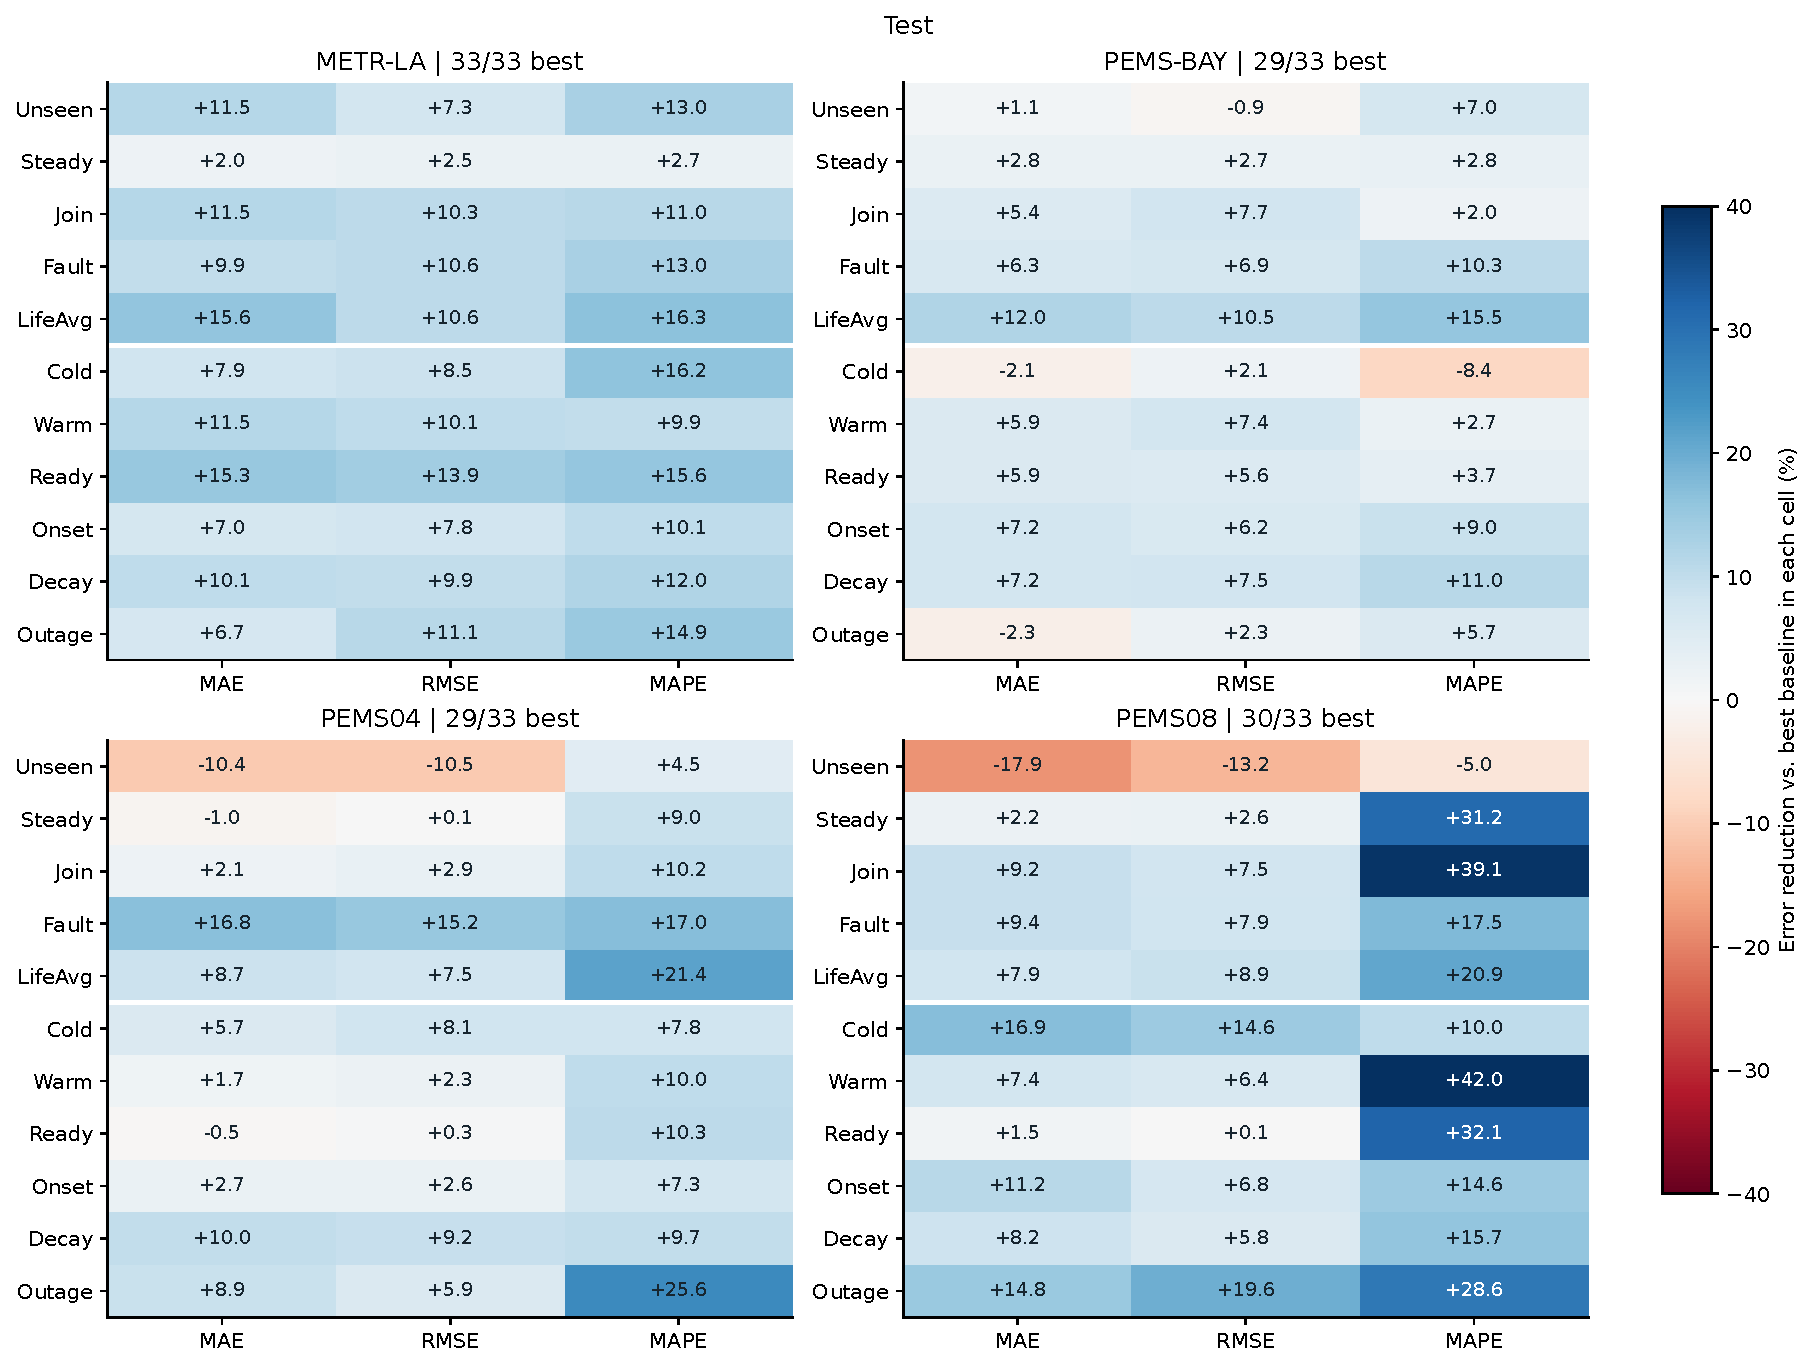
\includegraphics[width=\textwidth]{figures/fig2_condition_stage_test.pdf}
\caption{\textbf{四数据集的场景与阶段收益（测试集）。}数值为 $100\times(1-E_{\mathrm{ALFNet}}/\min_b E_b)$，正值表示优于八个基线中该格的最优者。四个面板共享对称色标，保留全部正负收益；每个面板上部为四类场景与 LifeAvg，下部为 Join 与 Fault 的阶段。}
\label{fig:condition}
\end{figure}

ALFNet 在 METR-LA、PEMS-BAY、PEMS04、PEMS08 上分别取得33/33、29/33、29/33、30/33项第一。最稳定的结果出现在本地证据逐步形成或被打断的场景：Join 与 Fault 的三项指标在四个数据集上均优于所列八个基线，说明当保留节点开始提供少量观测、或已知节点失去近期读数时，条件化的信息利用能够持续带来收益。这与引言提出的预测要求一致：Join 场景需要在有限的本地证据与空间上下文之间协调，Fault 场景则需要在历史连续性降低后维持预测依据。

边界同样清晰。在没有任何本地历史的 Unseen 场景下，优势依赖于数据集：METR-LA 上三项指标均为第一，PEMS-BAY 上 MAE 与 MAPE 为第一而 RMSE 比该指标最强基线高0.9\%；流量数据上，PEMS04 的 MAE 与 RMSE 分别高10.4\%和10.5\%（MAPE 仍降低4.5\%），PEMS08 的三项误差分别高17.9\%、13.2\%和5.0\%。其余未取得第一的格子集中在本地历史接近缺失的端点（PEMS-BAY 的 Cold 与 Outage），以及 PEMS04 中 Steady 与 Ready 的 MAE（差距分别为1.0\%和0.5\%）。因此，流量数据上的收益主要来自本地证据存在或部分存在时对历史与空间信息的利用，Unseen 场景的泛化则是另一类问题。

\subsection{条件化组件的贡献（RQ2）}\label{sec:4_4}

表\ref{tab:ablation}显示，跨节点时间上下文与时间条件分支对预测收益的贡献最大，由生命周期上下文决定的空间路由与状态进度带来幅度较小的改进。在本次运行中，移除 Adaptive Routing、Spatial Context 或 ALFTemporal–FiLM 均使四个数据集的三项 LifeAvg 变差；移除 State Progress 在12个数据集—指标格中使11格变差。所有变体与对应完整模型共享超参数、随机种子、数据划分和检查点准则。

\begin{table}[t]
\caption{\textbf{四数据集四项组件消融（测试集 LifeAvg）。}每行为一个变体，各数据集每项指标的最优值加粗、次优值加下划线，按未舍入值排名。}
\label{tab:ablation}
\centering
\small
\setlength{\tabcolsep}{3pt}
\resizebox{\linewidth}{!}{% Generated by _scripts/make_tables.py from frozen result files; do not edit by hand.
\begin{tabular}{lrrrrrrrrrrrr}
\toprule
\multirow{2}{*}{变体} & \multicolumn{3}{c}{METR-LA} & \multicolumn{3}{c}{PEMS-BAY} & \multicolumn{3}{c}{PEMS04} & \multicolumn{3}{c}{PEMS08} \\
\cmidrule(lr){2-4} \cmidrule(lr){5-7} \cmidrule(lr){8-10} \cmidrule(lr){11-13}
 & MAE$\downarrow$ & RMSE$\downarrow$ & MAPE(\%)$\downarrow$ & MAE$\downarrow$ & RMSE$\downarrow$ & MAPE(\%)$\downarrow$ & MAE$\downarrow$ & RMSE$\downarrow$ & MAPE(\%)$\downarrow$ & MAE$\downarrow$ & RMSE$\downarrow$ & MAPE(\%)$\downarrow$ \\
\midrule
ALFNet & \textbf{3.842} & \textbf{6.085} & \textbf{10.337} & \textbf{2.723} & \textbf{4.201} & \textbf{6.276} & \textbf{39.565} & \underline{53.346} & \textbf{23.257} & \textbf{36.780} & \textbf{46.567} & \textbf{43.000} \\
w/o State Progress & \underline{3.878} & \underline{6.097} & \underline{10.423} & \underline{2.732} & \underline{4.248} & \underline{6.464} & \underline{39.757} & \textbf{53.136} & 24.957 & \underline{38.162} & \underline{47.792} & \underline{48.701} \\
w/o Adaptive Routing & 3.920 & 6.127 & 10.602 & 2.770 & 4.280 & 6.514 & 39.826 & 53.401 & \underline{23.415} & 38.783 & 49.591 & 58.378 \\
w/o Spatial Context & 4.400 & 6.645 & 12.529 & 2.958 & 4.493 & 7.011 & 40.292 & 54.694 & 24.877 & 42.382 & 53.475 & 53.061 \\
w/o ALFTemporal–FiLM & 4.264 & 6.560 & 11.760 & 2.890 & 4.487 & 6.992 & 42.137 & 56.293 & 26.361 & 40.906 & 51.874 & 52.003 \\
\bottomrule
\end{tabular}
}
\end{table}

在表\ref{tab:ablation}所列四项消融中，完整模型在 METR-LA、PEMS-BAY 与 PEMS08 上三项指标均最优，在 PEMS04 上取得 MAE 与 MAPE 最优；唯一例外是 PEMS04 的 w/o State Progress 的 RMSE（53.136，较完整模型低0.39\%）。本文按观测值报告，未将小差异解释为统计显著。

\textbf{跨节点上下文与时间条件分支贡献最稳定。} w/o Spatial Context 保持参数规模不变，只让同一组时间处理模块逐节点工作，不再利用跨节点分区上下文；其 MAE 增幅在四个数据集上为1.84\%–15.23\%，在 METR-LA 与 PEMS08 上超过14\%。w/o ALFTemporal–FiLM 移除整个时间条件分支及其调制，MAE 增幅为6.1\%–11.2\%。前者排除了“单纯参数增多”的解释，后者说明完整分支对预测有实质作用；两项干预的范围有重叠，不视作互不相关的贡献相加。

\textbf{OS 条件化的传播在本次运行的四个数据集上均降低误差。} w/o Adaptive Routing 保留五种传播支持，仅以与输入无关的全局可学习混合替代由生命周期上下文决定的路由，四个数据集的三项误差均上升；除 PEMS08 外，上升幅度为0.10\%–3.80\%，PEMS08 的 MAPE 增幅则达35.76\%。在传播算子不变的前提下，随 OS 变化的组合方式仍然有益，支持依据 OS 调整空间信息交换的设计。

\textbf{状态进度提供补充性的阶段区分信息。} w/o State Progress 用掩码替代状态进度通道并保留观测角色输入，在 METR-LA、PEMS-BAY 和 PEMS08 上使三项指标同时上升，在 PEMS08 上对 MAPE 的影响尤为明显（增幅13.26\%）。这支持状态进度在不同历史阶段之间提供区分信息；PEMS04 的 RMSE 例外说明该补充并非在所有误差尺度上同等重要，也不能由这一干预单独推断观测角色编码本身的贡献。

\subsection{观测轨迹下的预测响应（RQ3）}\label{sec:4_5}

条件平均无法区分交通目标变化和观测变化的影响。为隔离 OS 变化，每个数据集固定64个历史与未来自然完整的已知节点验证窗口，保持预测目标、图结构和其他节点输入不变，只干预焦点节点；样本按固定随机规则选取，不依据预测误差筛选。加入干预保留最近3步或6步，以完整12步为参照；中断干预删除最近3步、6步或全部历史，并同步更新观测角色与状态进度。模型参数固定，因此结果反映对可用证据的响应而非在线学习效果；这是已知节点上的受控输入实验，不等同于保留节点上的 Join 或 Unseen 场景。

对比的代表基线按各数据集完整验证集 LifeAvg MAE 在三类方法中各取最优：前两类为 UIGNN 与 MoGERNN，第三类在速度数据上为 STBP，在流量数据上为 PatchSTG。后文\ref{sec:4_6}与\ref{sec:4_8}沿用这一选择。图\ref{fig:trajectory}、图\ref{fig:layout}与图\ref{fig:cases}均使用与表\ref{tab:main}一致的最终权重；正文统一展示验证集，按相同抽样与干预规则得到的测试集结果在\ref{sec:4_8}节末段核验。两套结果完整保留，不在不同图或数据集之间按结果择优切换划分。

\begin{figure}[t]
\centering
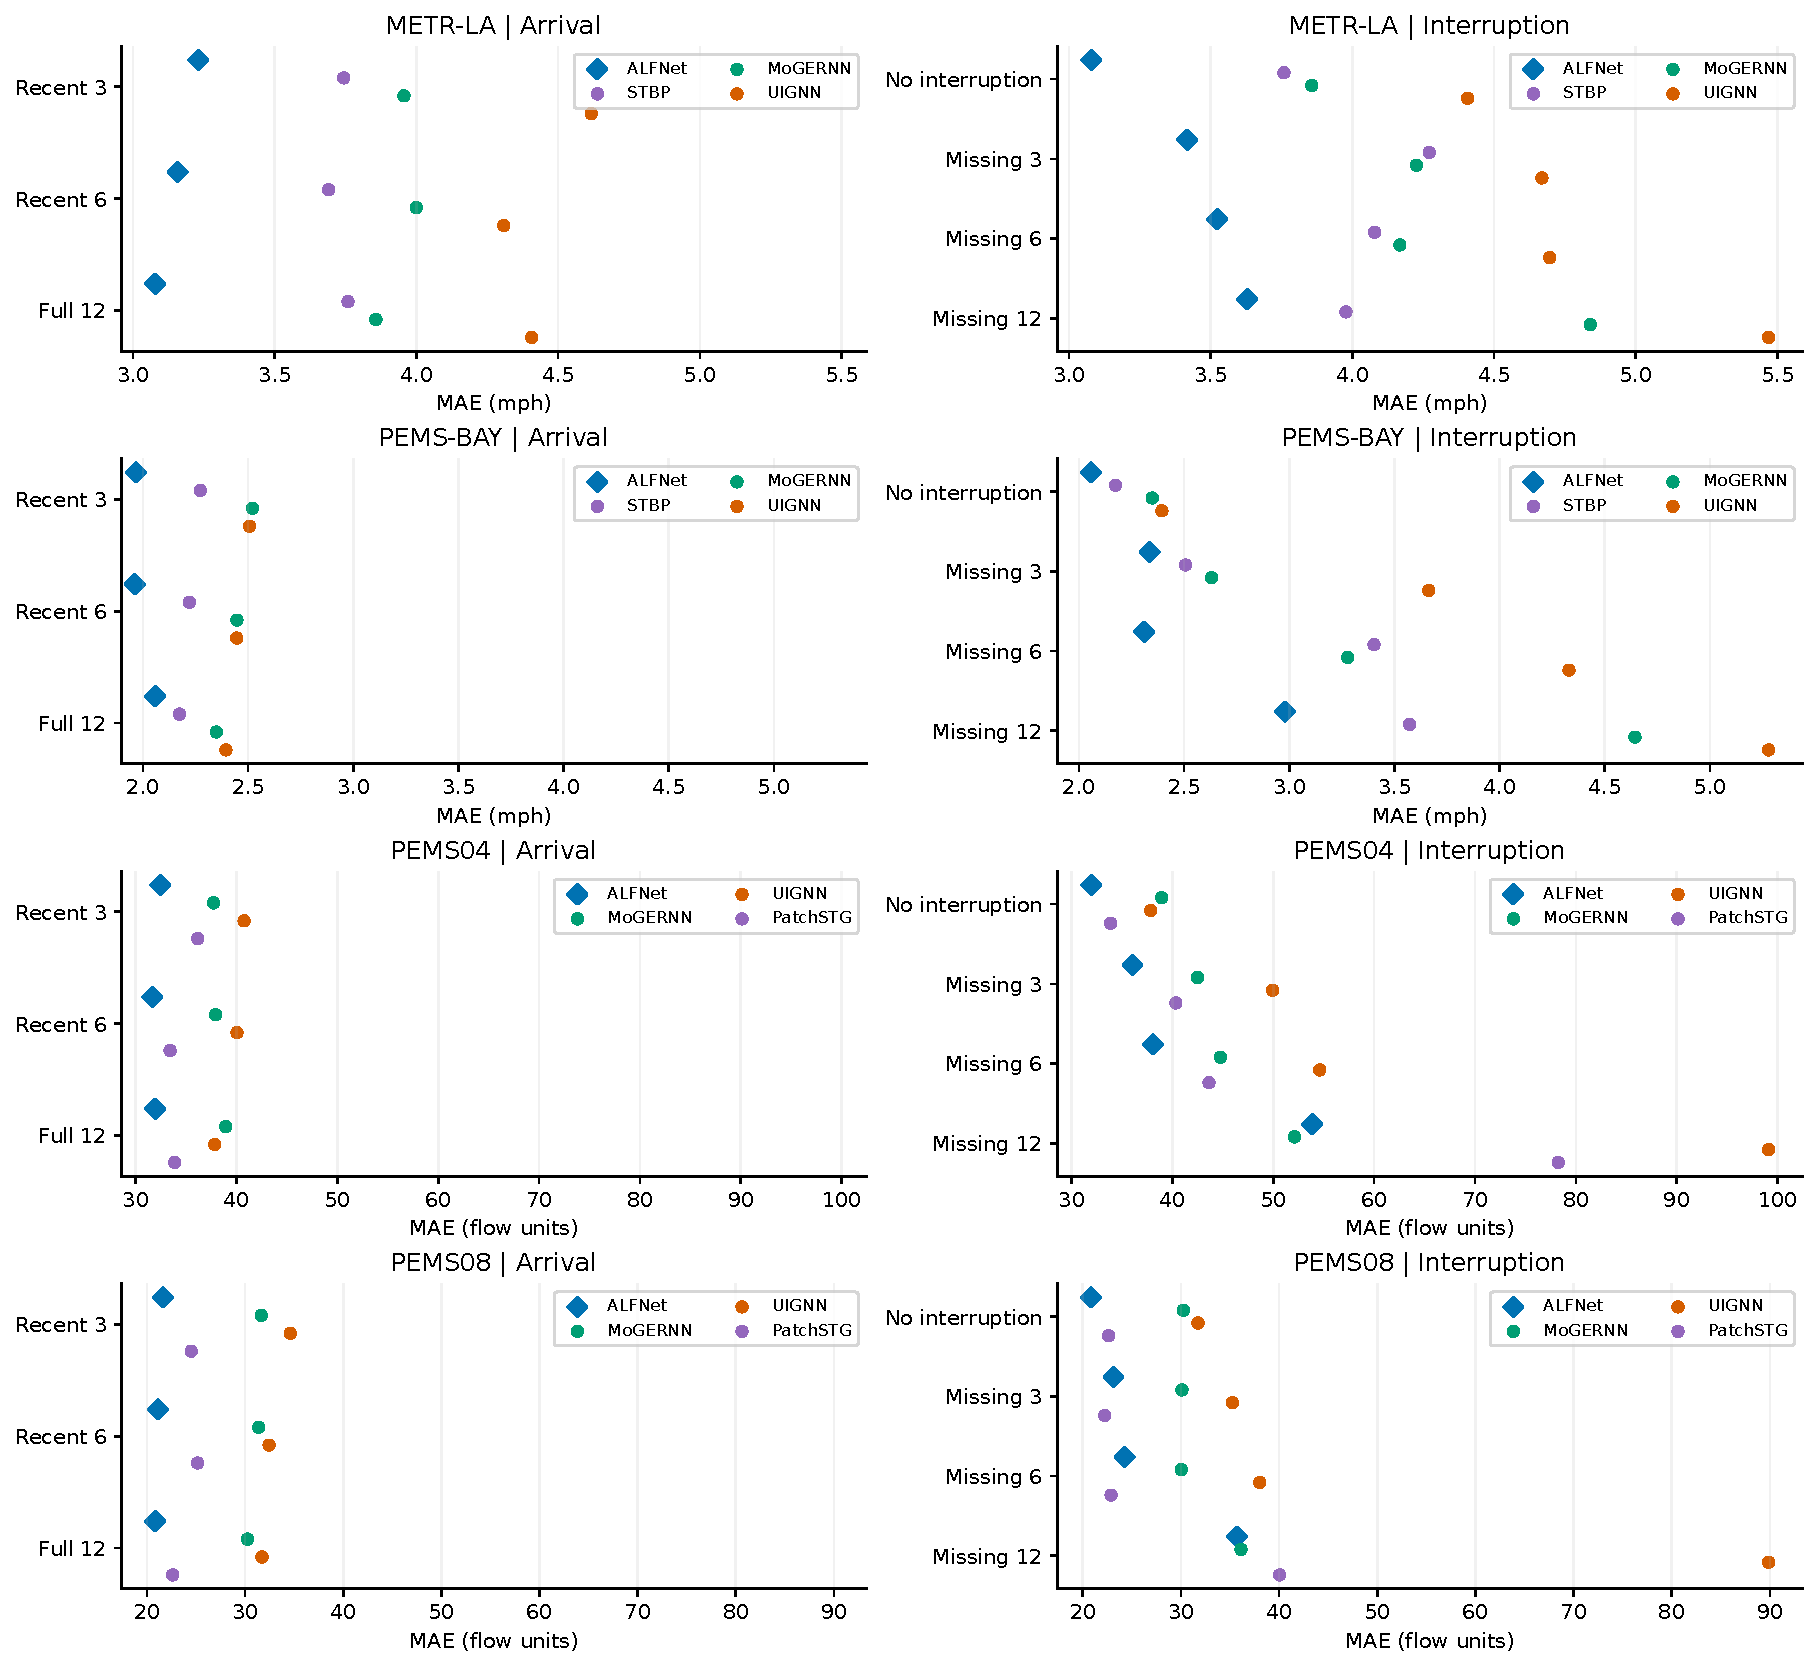
\includegraphics[width=\textwidth]{figures/fig3_trajectory_val.pdf}
\caption{\textbf{固定目标下的观测加入与中断（验证集）。}每行为一个数据集，左列为加入，右列为中断。点为同一组64个窗口、全部12个预测步上的平均 MAE，越靠左越好；同一行共享横轴尺度，离散干预点不连成在线学习曲线。}
\label{fig:trajectory}
\end{figure}

在加入干预下，ALFNet 在四个数据集的三个设置中均低于三个代表基线，其误差在 METR-LA 与 PEMS08 上随近期历史增加而下降。在中断干预下，速度数据的全部设置中 ALFNet 保持最低误差，完全中断时 MAE 分别为3.628（METR-LA）和2.979（PEMS-BAY）；流量数据上，PEMS08 在完全中断时仍优于三个代表基线，PEMS04 则在部分历史可用时保持优势，完全中断端点略高于 MoGERNN。PEMS08 的部分中断劣于 PatchSTG：中断3步与6步时 MAE 分别为23.126／22.232和24.270／22.880，误差高约4.0\%与6.1\%，因此不能概括为所有中断强度均占优。整体上，新增本地观测的利用与失去本地观测后的空间补偿共同决定模型响应，而不是单一的缺失率决定性能。这些受控响应与条件化设计相符，可与表\ref{tab:ablation}的消融结果结合理解。

\subsection{观测数量与时间布局（RQ3）}\label{sec:4_6}

相同数量的观测并不提供相同的信息。沿用图\ref{fig:trajectory}的配对窗口，固定 AAS 观测角色与状态进度，只改变可见读数在12步历史中的位置：Recent 保留近期历史，Early 保留早期历史，Dispersed 分散保留，Middle Gap 保留中间连续缺口两侧的读数。所有布局只删除自然存在的读数，不合成新观测。

\begin{figure}[t]
\centering
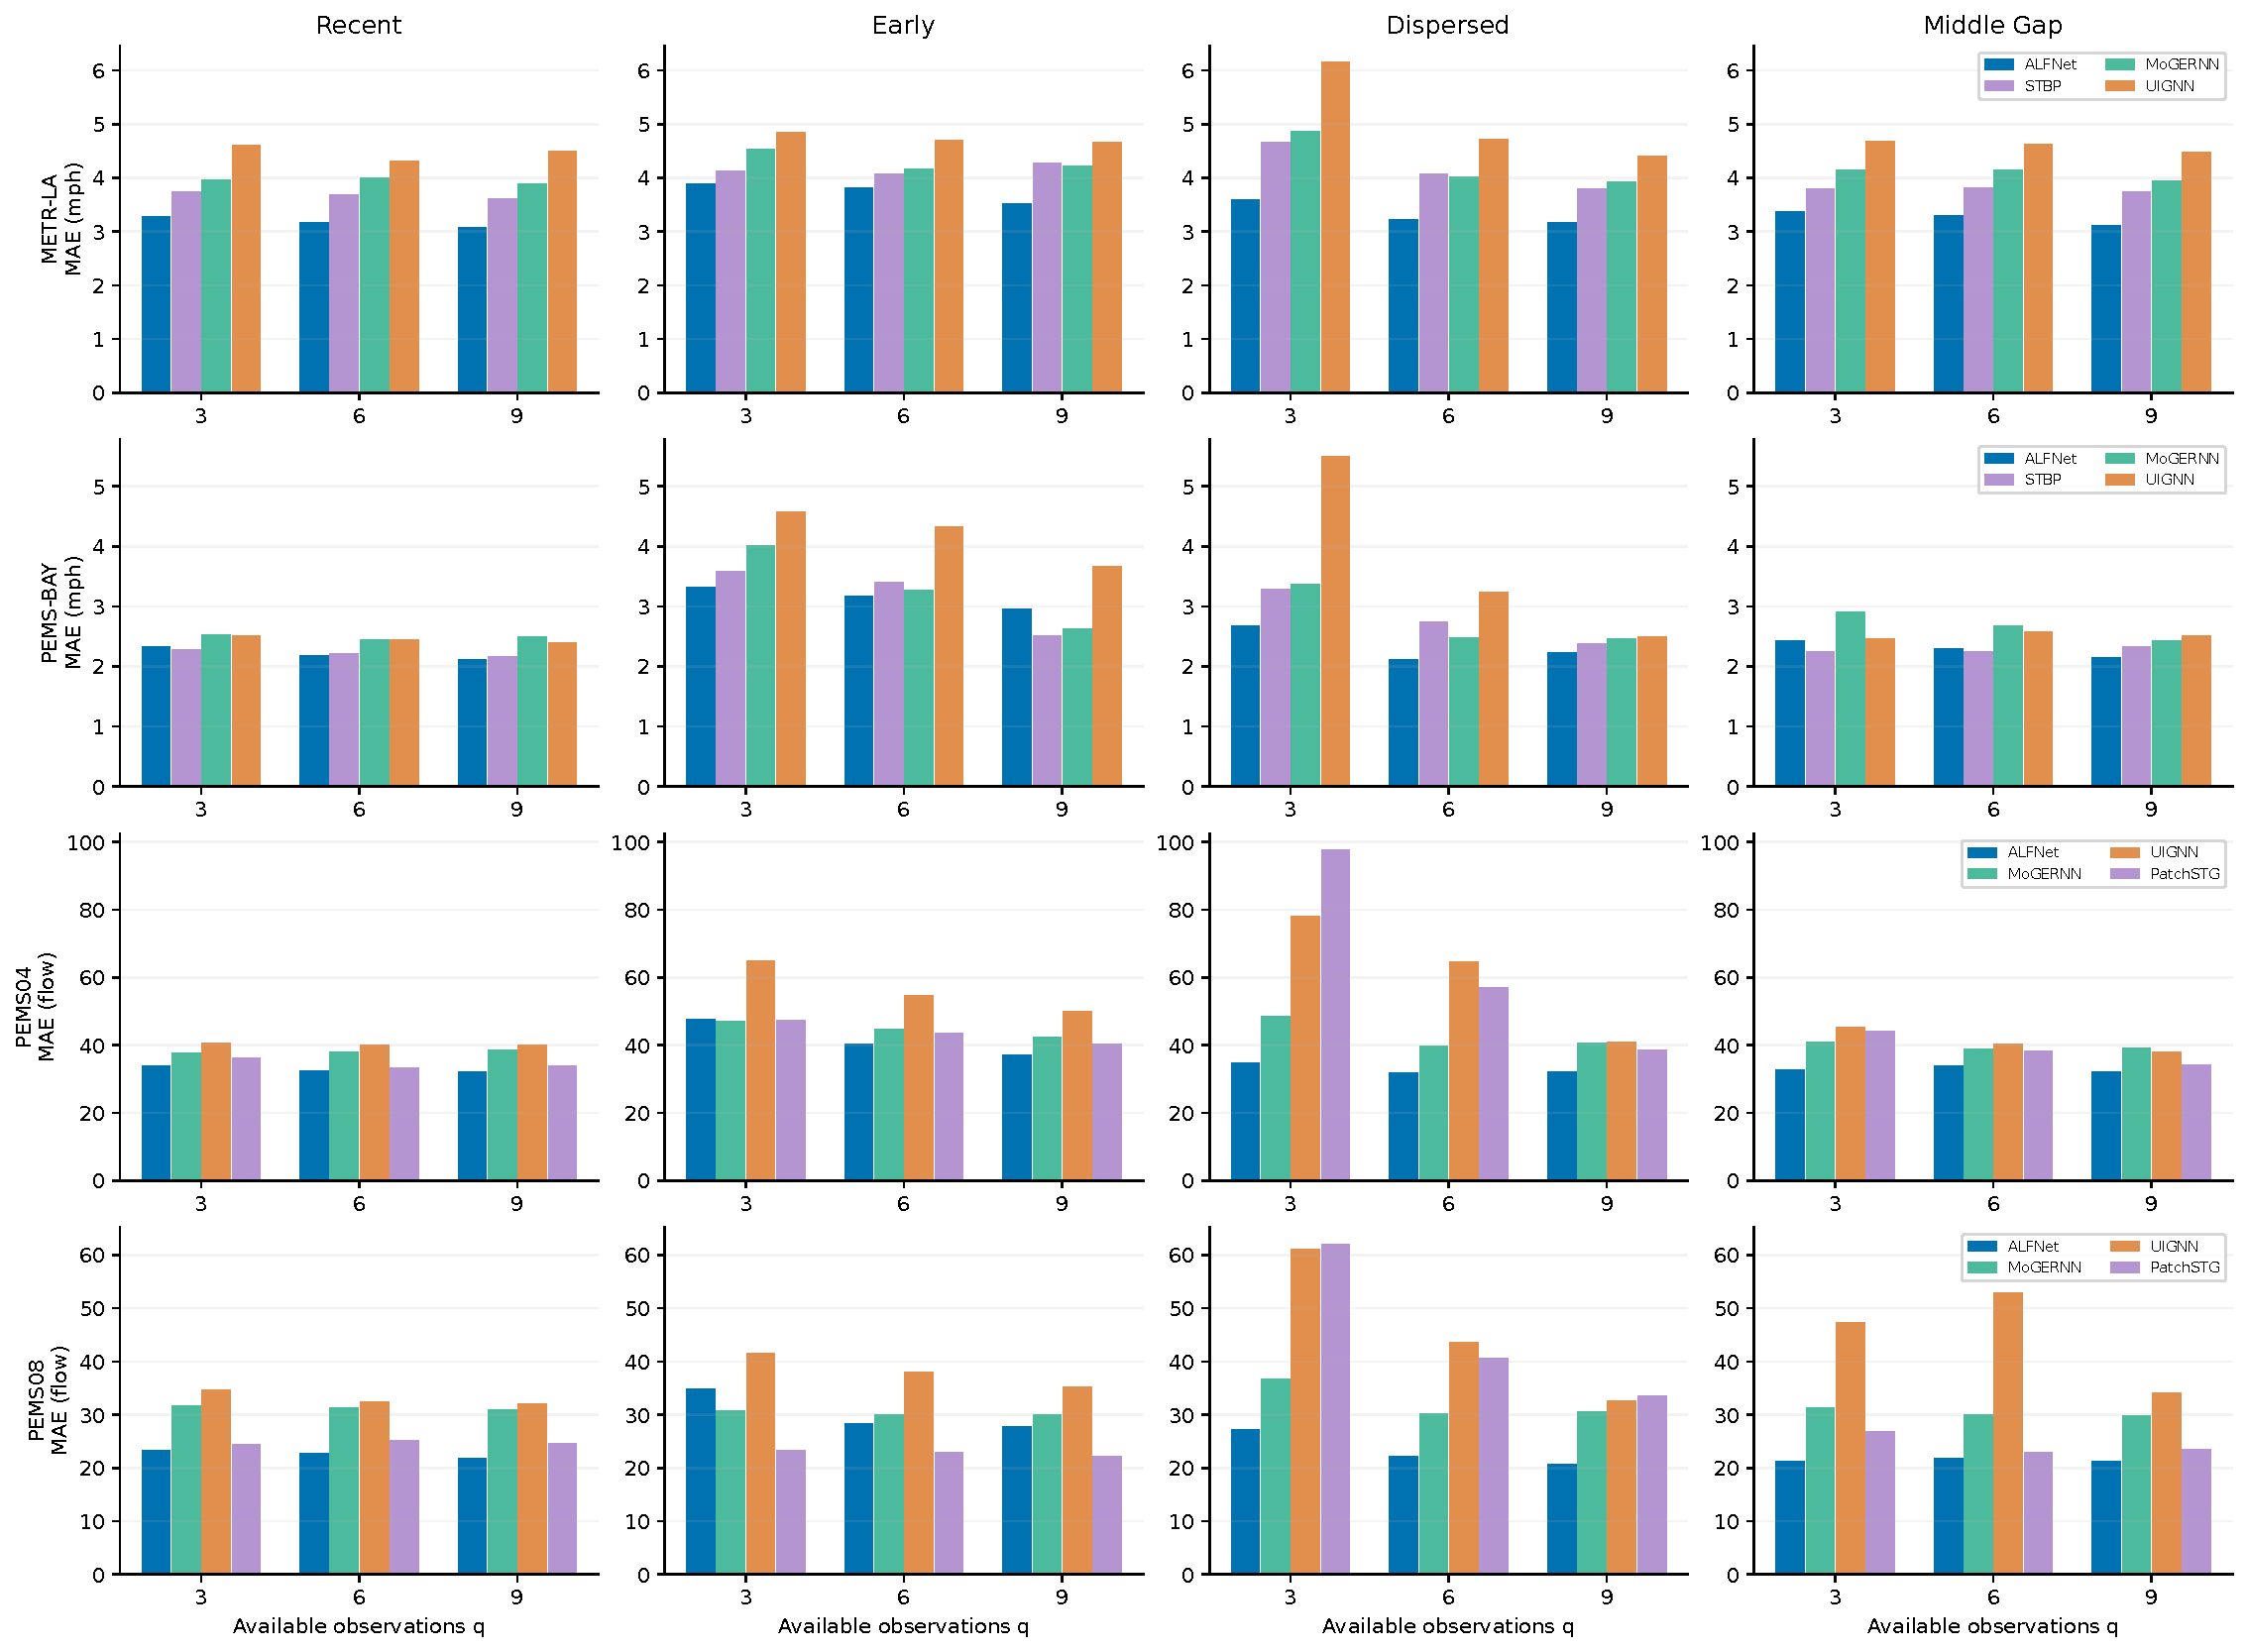
\includegraphics[width=\textwidth]{figures/fig4_layout_val.pdf}
\caption{\textbf{观测数量与时间布局的比较（验证集）。}行为数据集、列为布局，每组比较相同 $q=3,6,9$ 下的四个模型；柱轴从零开始，同一数据集的各布局共享尺度。共享端点 $q=0$ 与 $q=12$ 不在四种布局中重复展示。}
\label{fig:layout}
\end{figure}

四个数据集都体现出近期信息的价值：固定 $q=6$ 时，ALFNet 在 Recent 与 Early 布局下的 MAE 分别为3.164／3.808（METR-LA）、2.188／3.165（PEMS-BAY）、32.336／40.265（PEMS04）和22.822／28.404（PEMS08），Recent 一致更低。除 METR-LA 外，其余三个数据集上的分散历史略优于单独保留近期历史，说明新近程度与时间覆盖共同决定有效信息，单纯统计可见数量不足以刻画预测条件。这一观察对应引言的论点：观测数量只描述有多少信息，时间布局还决定信息来自何时。

在各数据集12个数量—布局组合中，ALFNet 分别在12、8、11、9个组合上取得最低 MAE，收益覆盖近期、分散与连续缺口等不同模式。未取得最低的组合主要出现在 PEMS-BAY（由 STBP 取得）以及 PEMS08 的 Early 布局（由 PatchSTG 取得），即该布局中最近观测缺失、仅保留早期读数的情形；这与\ref{sec:4_3}中优势在本地证据偏弱时更不稳定的观察方向一致。

\subsection{超参数敏感性}\label{sec:4_7}

在各数据集固定锚点上，每次只改变分区容量、学习率倍率、ALFTemporal dropout 或 AdamW 权重衰减中的一项，其余设置不变。所有配置以相同种子训练，并按验证集 LifeAvg MAE 选择检查点。速度数据复用已完成的固定锚点实验，流量数据使用最终插值、倍率与中心化方案下的单因素实验。

\begin{center}
\small
\resizebox{\linewidth}{!}{% Generated by _scripts/make_tables.py from frozen result files; do not edit by hand.
\begin{tabular}{llllll}
\toprule
数据集 & 锚点（容量／LR／dropout／权重衰减） & 容量候选 & LR 候选 & dropout 候选 & 权重衰减候选 \\
\midrule
METR-LA & 8／1／0.1／$10^{-4}$ & 7、8、10、12 & 0.5、1、2 & 0.05、0.1、0.2 & $10^{-5}$、$10^{-4}$、$10^{-3}$ \\
PEMS-BAY & 16／1／0.1／$10^{-4}$ & 11、12、14、16 & 0.5、1、2 & 0.05、0.1、0.2 & $10^{-5}$、$10^{-4}$、$10^{-3}$ \\
PEMS04 & 10／1／0.1／$10^{-4}$ & 10、14、18 & 0.5、1、2 & 0.05、0.1、0.2 & $10^{-5}$、$10^{-4}$、$10^{-3}$ \\
PEMS08 & 6／1／0.1／$10^{-4}$ & 6、8、10 & 0.5、1、2 & 0.05、0.1、0.2 & $10^{-5}$、$10^{-4}$、$10^{-3}$ \\
\bottomrule
\end{tabular}
}
\end{center}

\begin{figure}[t]
\centering
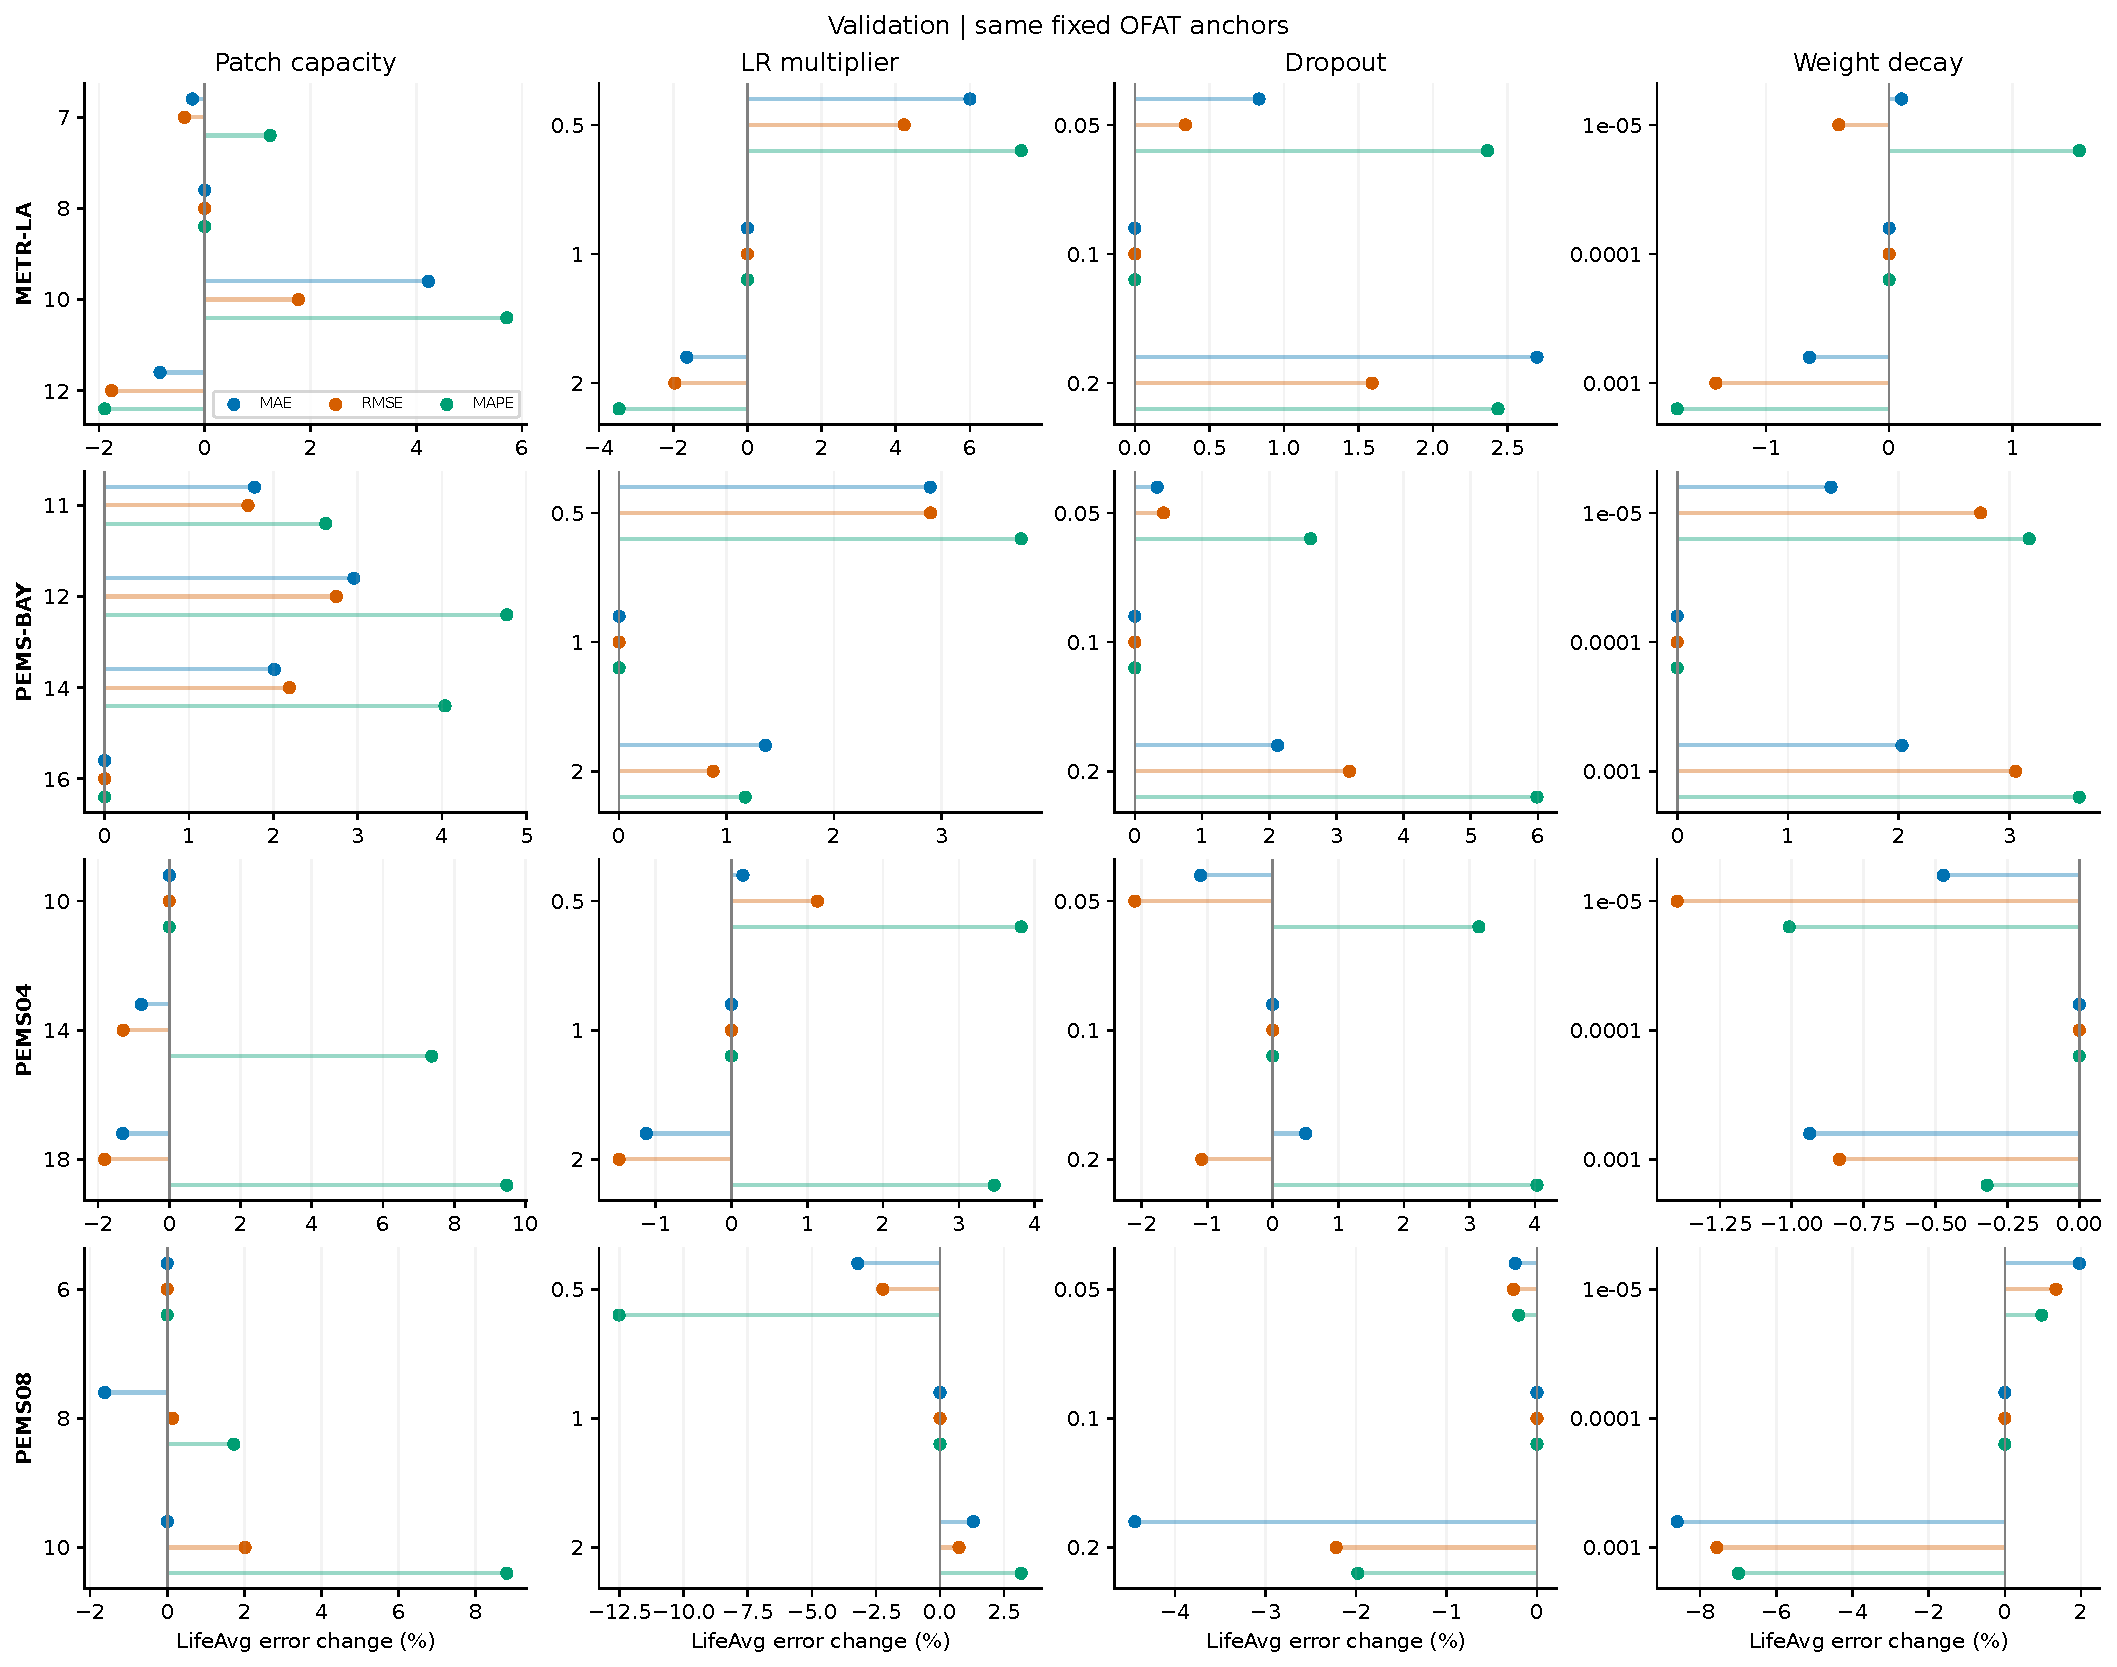
\includegraphics[width=\textwidth]{figures/fig5_hyperparameters_val.pdf}
\caption{\textbf{单因素敏感性（验证集）。}行为数据集、列为参数；每个参数值用三种颜色表示 LifeAvg MAE、RMSE、MAPE 相对本数据集锚点的百分比变化。零线为锚点，负值更优；线段连接零线与实测值，不表示参数间插值或置信区间。}
\label{fig:hparam}
\end{figure}

参数作用具有数据集依赖性。速度数据上，MAE 的变化多在3\%以内，例外是 METR-LA 的学习率减半（MAE 上升6.00\%）与容量10（上升4.23\%）；两个数据集均在 dropout 0.1 下取得三项指标的最低值。PEMS-BAY 的锚点容量16为所测最大值，较小容量在三项指标上均变差，说明该数据集上更大的分区容量有利。流量数据则呈现更明显的容量—误差尺度取舍：PEMS04 增大容量降低 MAE 与 RMSE，却使 MAPE 上升（容量18时约上升9.5\%）；PEMS08 对正则化更敏感，权重衰减 $10^{-3}$ 将三项指标分别降低8.60\%、7.56\%和6.99\%。

部分非锚点配置在验证集上优于锚点（如 METR-LA 的学习率加倍），因此单因素实验只用于说明各参数的作用，误差变化均相对本数据集锚点计算。

\subsection{样本层面的预测行为（RQ4）}\label{sec:4_8}

为观察本地历史完全不可用时预测如何偏离真实值，我们将分析分为全部窗口的误差分布与具体预测目标两部分。图\ref{fig:cases}使用图\ref{fig:trajectory}相同的64个已知节点窗口，在完全中断干预下比较各模型。

\begin{figure}[t]
\centering
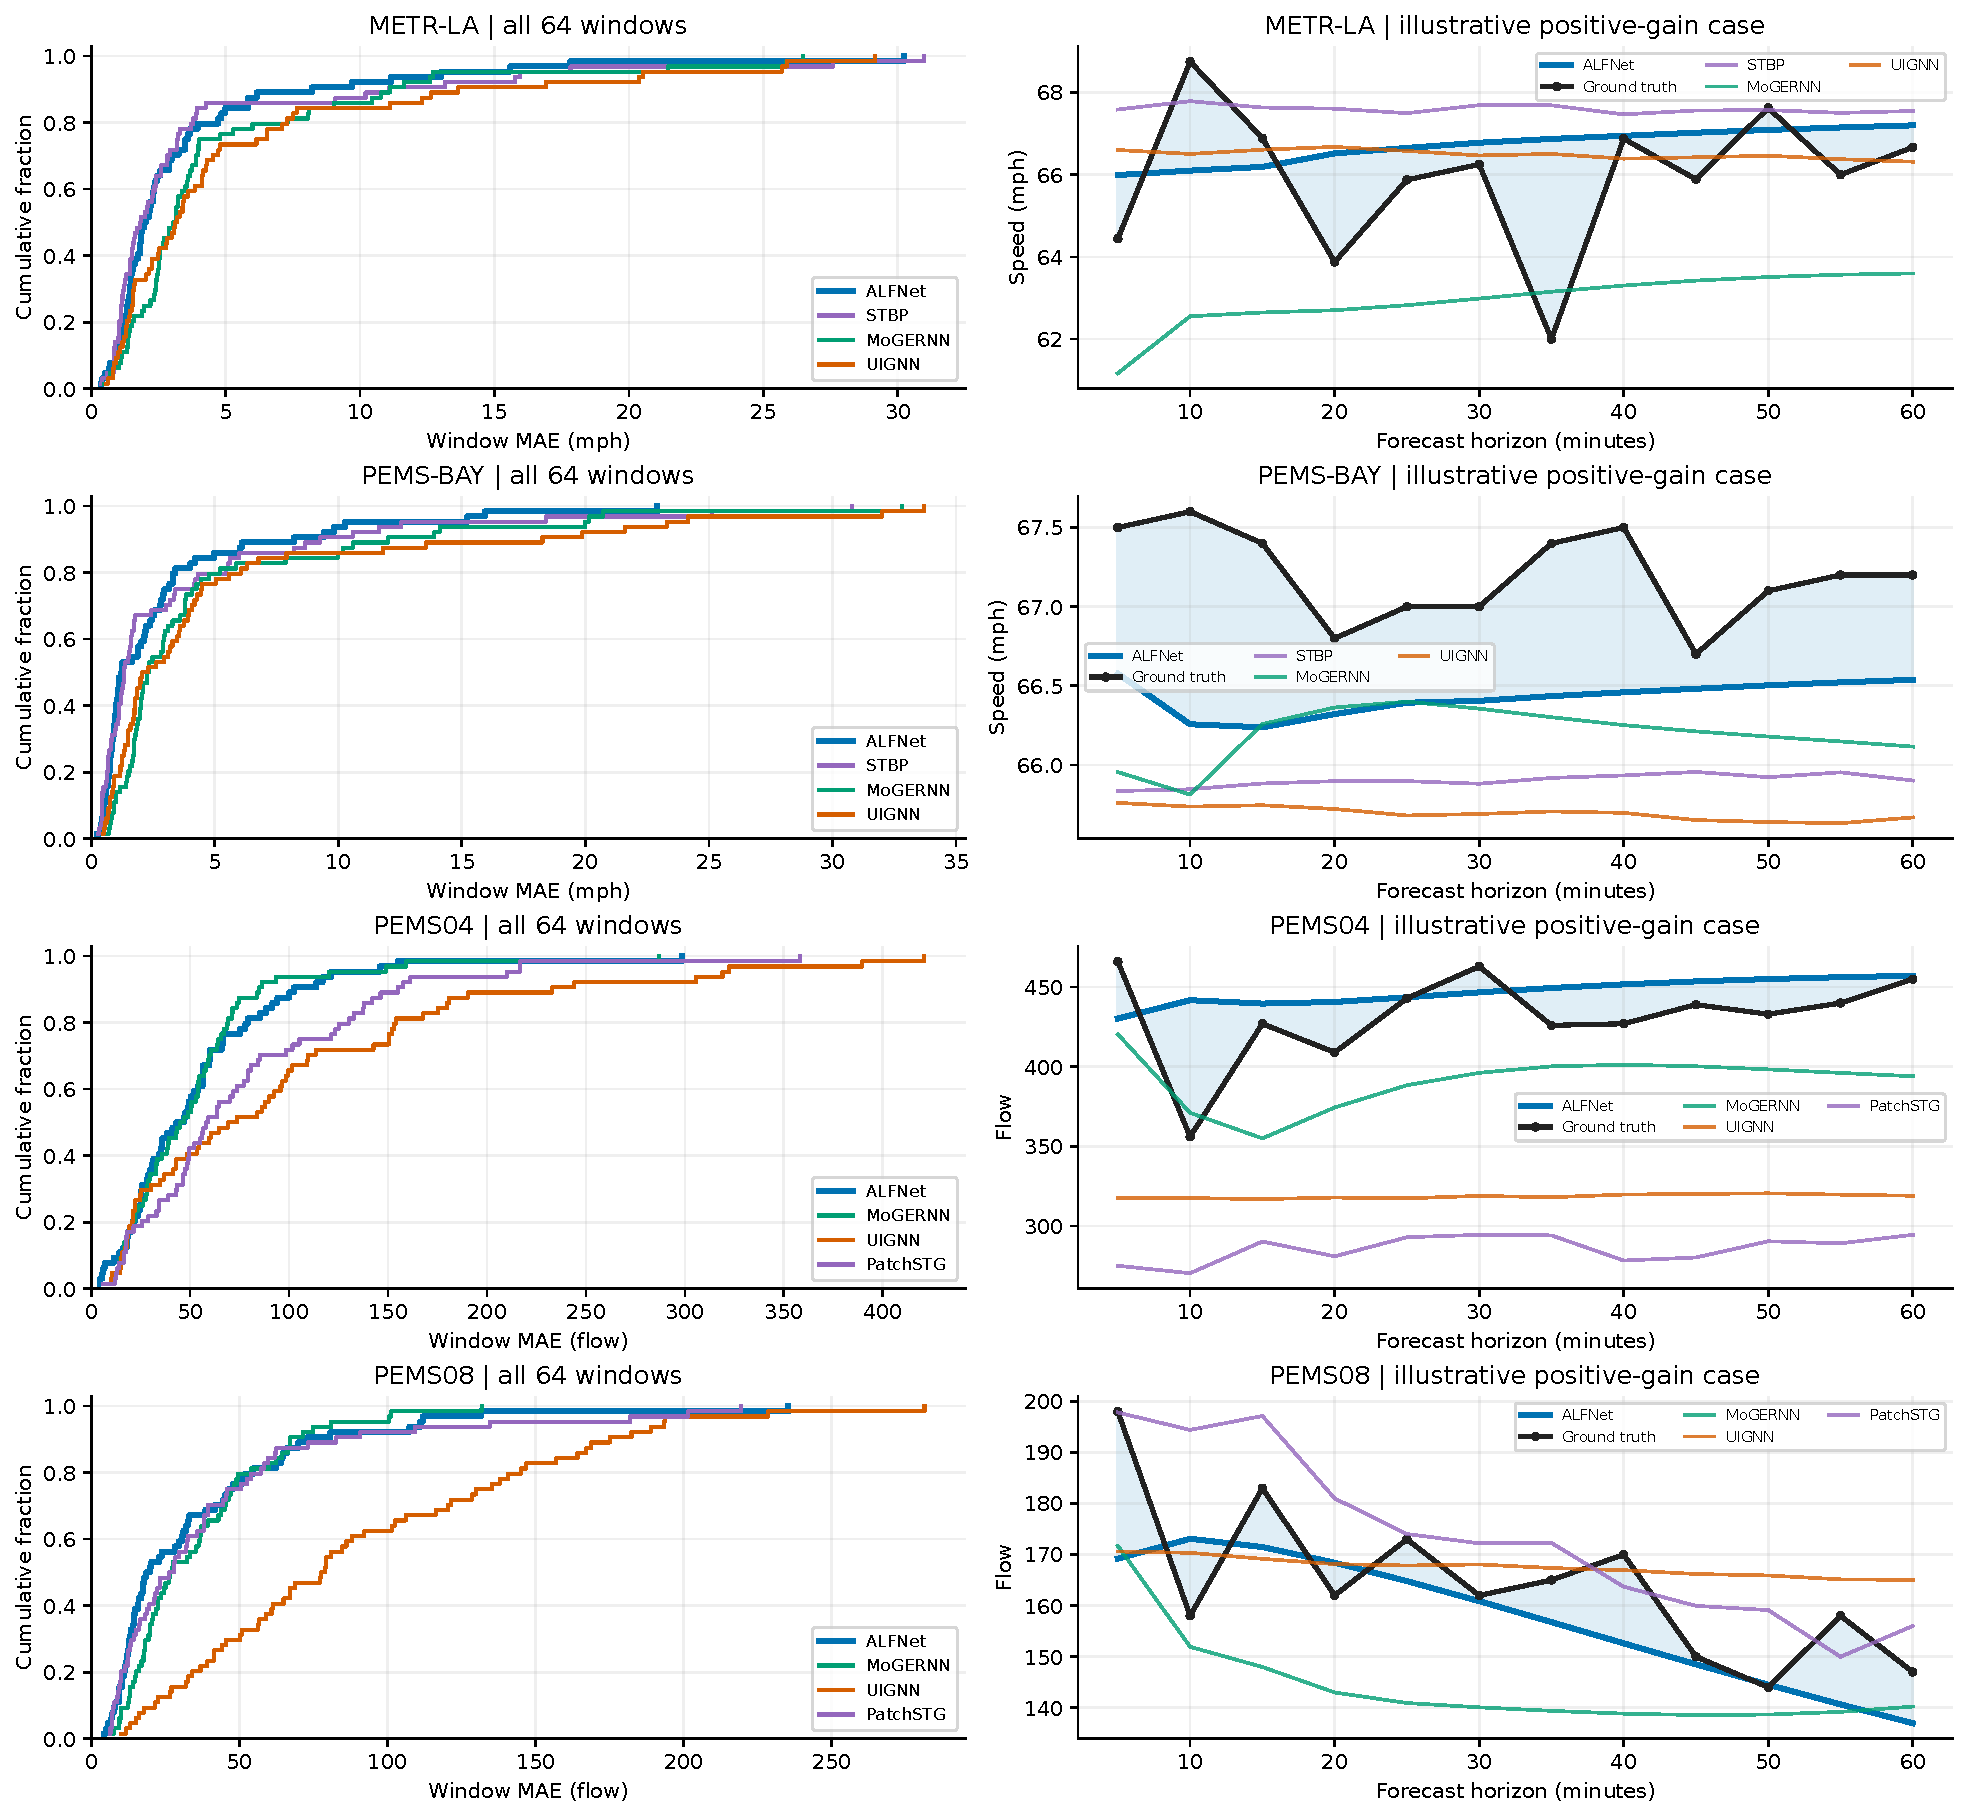
\includegraphics[width=\textwidth]{figures/fig6_cases_val.pdf}
\caption{\textbf{完全中断干预下的分布与案例分析（验证集）。}左列为全部64个窗口 MAE 的经验累积分布，同一误差阈值下曲线越高表示更多窗口达到该精度，不截去大误差。右列为优势示例：先确定本数据集该干预下平均 MAE 最低的代表基线，再从 ALFNet 优于它的窗口中选取收益最接近正收益中位数的一个。该选择用于展示实际存在的优势，不代表随机案例或总体胜率；黑线为真值，浅蓝色带为 ALFNet 与真值的差距，不是置信区间。}
\label{fig:cases}
\end{figure}

从分布看，速度数据上 ALFNet 的窗口 MAE 第90百分位均低于三个代表基线，表明速度数据的总体收益包含对较大窗口误差的控制。相对该干预下平均 MAE 最低的代表基线，ALFNet 在四个数据集上的窗口胜率依次为54.7\%、51.6\%、50.0\%和62.5\%，说明总体平均排序不等同于逐窗口占优；仅由这些胜率不能推断所有数据集的收益均来自尾部误差抑制。案例曲线仅用于直观展示预测水平：PEMS04 示例中 ALFNet 较好地维持了真实流量区间，减轻了其他方法的持续低估；PEMS08 示例中其预测跟随流量下降趋势，并减轻部分基线持续低估的偏差。局部波动仍无法完全追随，但预测依据并未因焦点节点失去历史而消失。由于案例按正收益中位数选取，本文不据此推导逐样本结论。

\textbf{跨划分核验。} 在相同最终权重和抽样规则下，测试集图\ref{fig:trajectory}的四数据集六个唯一干预点均取得最低MAE；图\ref{fig:layout}的最优组合数依次为12、5、12、9，与验证集的12、8、11、9并不一致。因此，轨迹收益在测试集上得到补充支持，但布局优势具有样本和划分依赖性；两套结果不能通过逐图择优拼成一组结论。
